%========================================================================
% Modelo para elaboracao de textos academicos: TCC, dissertacoes e teses
% Elaborado pelo GISIS - Grupo de Imageamento Sismico e Inversão Sismica.
%========================================================================
\chapter{Revisão Bibliográfica}
\label{ch:revisaobibliografica}

A modelagem e tomografia sísmica são técnicas essenciais na exploração de recursos naturais subterrâneos e na caracterização da subsuperfície terrestre. A tomografia sísmica é um método não invasivo que permite mapear as propriedades físicas do subsolo através da análise das ondas sísmicas geradas por fontes controladas. Um dos principais desafios na tomografia sísmica é a obtenção de informações precisas sobre as trajetórias das ondas sísmicas e suas velocidades de propagação em diferentes camadas geológicas. Nesse sentido, a equação \textit{eikonal}  é uma ferramenta fundamental para a modelagem e inversão e imageamento sísmico, pois descreve as frentes de onda e permite calcular os tempos de percurso das ondas sísmicas. Neste capítulo é explorado a equação eikonal, três resoluções numéricas e sua aplicação na tomografia de refração. Ao explorar esses tópicos, este capítulo fornecerá abrangentes conceitos utilizados na geração dos resultados deste trabalho.

\section{Modelagem sísmica}

Muitos fenômenos físicos tem suas simplificações e condições para serem simulados computacionalmente. O método sísmico parte do princípio da propagação de ondas mecânicas geradas a partir de uma fonte explosiva, sendo registradas em receptores posicionados na superfície da terra ou no fundo marinho \cite{sheriff1995exploration, rosa2010analise}. Um modelo de propriedades físicas de subsuperfície é necessário para a simulação computacional. Considerando a simplificação da equação da onda para meios acústicos e isotrópicos, onde a propriedade do meio são as velocidades da onda P, as frentes de onda podem ser geradas para realizar estudos sintéticos experimentais. Existem formatos de solução para uma equação que rege um fenômeno físico, dois deles são o caso analítica e o caso numérico. A solução analítica de um problema mostra a resposta exata do fenômeno em condições específicas previamente estabelecidas e a solução numérica resolve o problema de forma geral para diversos cenários. No caso da modelagem sísmica, as condições estabelecidas se aplicam ao modelo de velocidade, resolvendo a equação em um modelo homogêneo ou com camadas plano paralelas sem variação lateral de velocidade.  

\subsection*{Equação da onda para meios acústicos}

A equação base para a simulação sísmica utilizando a simplificação para meios acústicos pode ser formulada da seguinte maneira
\begin{equation}
	\nabla^2u(\mathbf{x}, t) - \dfrac{1}{v^2(\mathbf{x})}\dfrac{\partial^2u(\mathbf{x}, t)}{\partial t^2} = f(t),	
	\label{wave_equation}
\end{equation}
\noindent onde $u(\mathbf{x},t)$ é o campo de pressão hidrostática, $t$ é o tempo de propagação e $\mathbf{x} = (x,y,z)$ são as variáveis do sistema de coordenadas para o caso 3D. $v(\mathbf{x})$ é o modelo de velocidade, $f(t)$ é uma função que determina o formato do pulso propagado e $\nabla^2 = \partial_x + \partial_y + \partial_z$ é o operador laplaciano. \citeonline{igel2017computational} mostra algumas formas de resolver a equação da onda numericamente de forma prática e aplicada. O método das diferenças finitas é um dos métodos mais utilizados em simulações sísmicas. O princípio do método é estimar o valor da derivada numericamente utilizando a série de Taylor, definida detalhadamente no trabalho de \citeonline{de2005funccoes}. Somente derivadas de segunda ordem são necessárias para resolver a equação \ref{wave_equation} e a aproximação da derivada pode ser definida a partir da seguinte expressão
\begin{equation}
	\dfrac{\partial^2 f(x)}{\partial x^2} \approx \dfrac{f[i - dh] - 2f[i] + f[i + dh]}{dh^2},
	\label{derivada_2}
\end{equation}    
\noindent onde $f(x)$ é uma função contínua arbitrária definida no eixo $x \in \mathbb{R}$ e $f[i]$ é uma função discreta definida na mesma reta com intervalos regulares $dh$. A equação da onda para meios acústicos pode ser escrita em seu formato discreto  substituindo a equação \ref{derivada_2} na equação \ref{wave_equation}, para cada eixo $x,y,z,t$ respectivamente. O método das diferenças finitas possui certas limitações como por exemplo a dispersão e instabilidade numérica \cite{aki1980quantitative}. Seguindo os trabalhos de \citeonline{mufti1990large, bulcao2004modelagem} e \citeonline{robertsson2012numerical} as condições para contornar problemas numéricos na modelagem sísmica para meios acústicos seguem na forma a seguir
\begin{equation}
	\begin{cases}
		dh \le v_{\text{min}} \,/\, (\alpha \cdot f_{\text{max}}) \\
		dt \le dh \,/\, (\beta \cdot v_{\text{max}})
	\end{cases}
\end{equation}   
\noindent onde $dh$ e $dt$ são os parâmetros de discretização espacial e temporal respectivamente, $v_{\text{min}}$ e $v_{\text{max}}$ são as velocidades da onda P mínima e máxima no modelo, $f_{\text{max}}$ é a frequência máxima da fonte sísmica aplicada, e $\alpha$ e $\beta$ são as quantidades de amostras para representar um comprimento de onda no espaço e no tempo respectivamente. Os valores de $\alpha$ e $\beta$ variam de acordo com a ordem do operador de diferenças finitas \cite{bulcao2004modelagem}.    

A fonte sísmica pode assumir diferentes formas dependendo de seu formato ou equacionamento. Na modelagem sísmica, a fonte é aplicada como um pulso definido no tempo discreto, onde a cada passo de tempo uma amostra do sinal é injetada, em uma posição no espaço, na resolução da equação da onda. A segunda derivada da equação gaussiana \cite{ricker1953form} pode ser usada para gerar o pulso sísmico, sendo definida da seguinte maneira
\begin{equation}
	\begin{cases}
		f_p = f_{\text{max}} / (3\sqrt{\pi}) \\
		g(t) = (1 - 2 \pi (\pi f_p t)^2) \exp(-\pi (\pi f_p t)^2)
	\end{cases}
\end{equation}
\noindent sendo $f_p$ a frequência de pico, $g(t)$ a fonte sísmica e $t$ o eixo do tempo. 

Ao contrário de dados sísmicos reais, onde o planeta absorve por completo a energia da onda, em simulação computacional, para os casos onde a equação da onda não contempla fenômenos dissipativos, existem técnicas para prevenir reflexões indesejadas causadas pelas bordas do modelo finito empregado. A condição de bordas absortivas de \citeonline{cerjan1985nonreflecting} é uma abordagem clássica para resolver o problema de bordas na modelagem sísmica, porém outras formulações mais elaboradas podem ser utilizadas, uma possibilidade é aplicar a formulação descrita no trabalho de \citeonline{chern2019reflectionless}. A condição de borda utilizada neste trabalho é regida pela equação a seguir
\begin{equation}
	w(\mathbf{x}) = exp(- p(n_b - \mathbf{x})^2),	
\end{equation}      
\noindent onde $w(\mathbf{x})$ é a função amortecimento definida somente nos pontos da borda $\mathbf{x}$, $p$ é um fator de atenuação e $n_b$ é a quantidade de amostras na borda. \citeonline{bording1921finite} compara experimentos para determinar valores otimizados para $n_b$ e $p$, em contrapartida \citeonline{gao2017comparison} mostram que a técnica esponjosa absortiva foi superada pelas novas variantes utilizando modificações da equação da onda. 

Utilizando a equação da onda em simulações sísmicas, alguns tipos de onda são registradas, que para o caso acústico escalar somente a onda P, porém existem as frentes de onda refletidas e refratadas. Nas próximas seções, somente as frentes de onda transmitidas e refratadas são exploradas pois esse tipo de onda é a ferramenta principal deste trabalho. As ondas refratadas acontecem quando o afastamento entre a fonte e o receptor são suficientemente grandes, dependendo da configuração de camadas geológicas em subsuperfície. Essas ondas refratadas comumente são chamadas de primeiras chegadas, pois se propagam em camadas de maior velocidade e assim são registradas em um tempo menor que as demais frentes de onda.          

\subsection*{Equação \textit{eikonal}}

A equação eikonal pode ser definida como uma aproximação de altas frequências para a equação da onda em meios acústicos. Essa definição pode ser expandida para outras simplificações de meio, como por exemplo o meio elástico isotrópico \cite{cerveny2003seismic}. \citeonline{rawlinson2008seismic} mostram as etapas de simplificação partindo da equação \ref{wave_equation}, assumindo uma solução periódica envolvendo tempo e frequência angular, aplicando essa solução na equação da onda, simplificando os termos e aplicando o limite da frequência angular tendendo ao infinito. Assim, a equação eikonal em três dimensões segue no formato 
\begin{equation}
	\left[\dfrac{\partial T(\mathbf{x})}{\partial x}\right]^2 + \left[\dfrac{\partial T(\mathbf{x})}{\partial y}\right]^2 + \left[\dfrac{\partial T(\mathbf{x})}{\partial z}\right]^2 = \dfrac{1}{v^2(\mathbf{x})} 	
\end{equation} 
\noindent sendo $T(\mathbf{x})$ a função tempo de trânsito avaliada na posição $\mathbf{x} = (x,y,z)$ e $s = 1/v$ pode ser chamado de vagarosidade, o inverso da velocidade. 





\subsection*{Equação analítica para ondas refratadas}

livro do kearey \cite{kearey2002introduction}



\begin{equation}
	t_n = \dfrac{x}{v_n} + \displaystyle\sum_{i=1}^{n-1} 2z_i cos(\theta_{in})
\end{equation}

\begin{figure}[H]
	\centering
	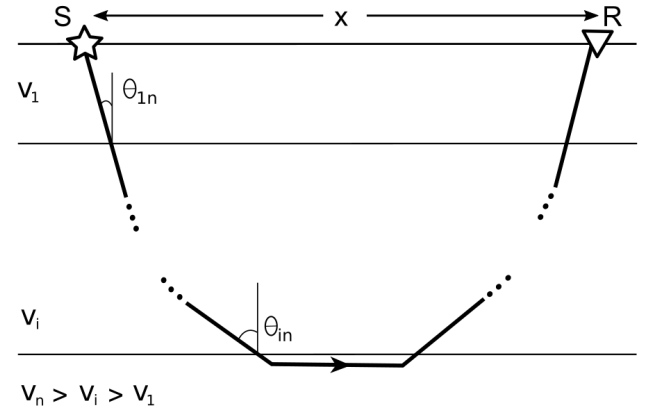
\includegraphics[width = 11cm, height = 7cm]{Imgs/RevisaoBibliografica/refracted_analytic.png}
	\caption{}
	\label{fig:refracted_analytic}
\end{figure}



\subsection*{Método clássico}

\cite{vidale1988finite}
\cite{podvin1991finite}
\cite{afnimar2000finite}
\cite{tryggvason2006travel}

desenvolvimento com o algoritmo time3d








\subsection*{\textit{Fast Iterative Method}}

\cite{jeong2008fast}
\cite{sethian1999fast}

\cite{fu2011fast, fu2013fast}

\cite{dang2014fast, hong2016multi, hong2022mg}

\cite{cai2023improved}

desenvolvimento com a implementação 






\subsection*{\textit{Fast Sweeping Method}}

original fast sweeping method

\cite{zhao2005fast}

\cite{zhao2007parallel}

\cite{detrixhe2013parallel}

\cite{noble2014accurate}


\subsection*{Comparação numérica}


\begin{figure}[H]
	\centering
	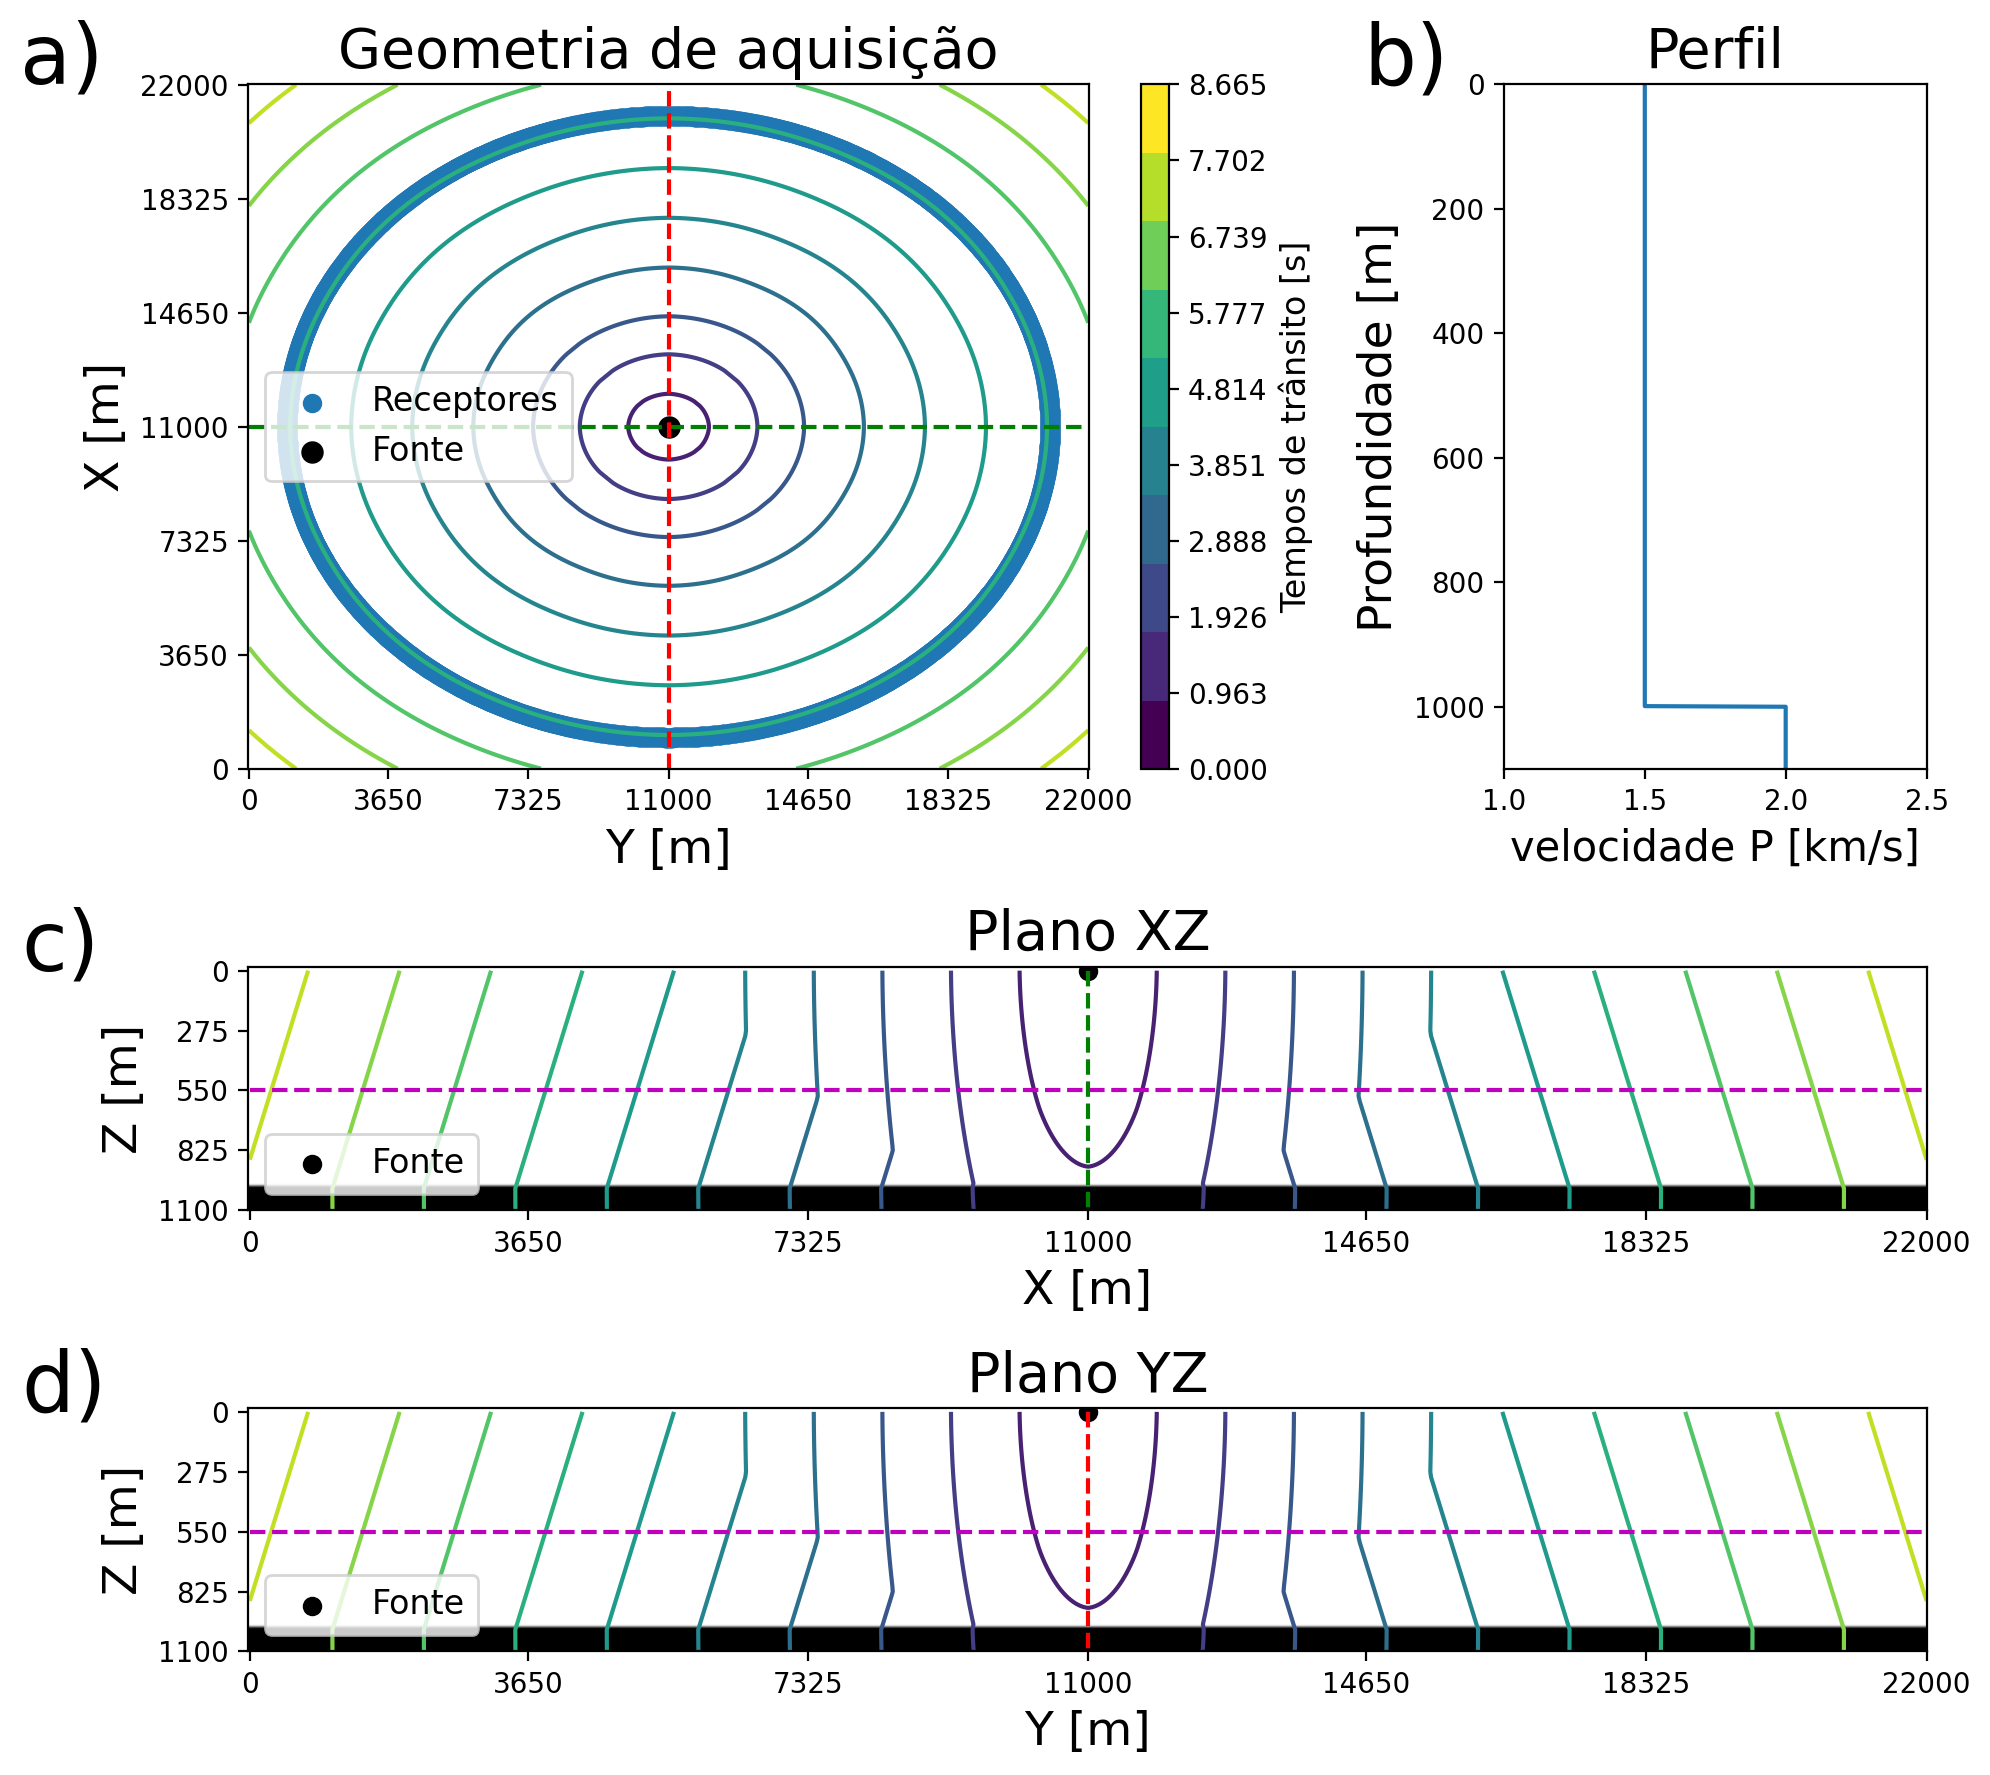
\includegraphics[width = 11cm, height = 10cm]{Imgs/RevisaoBibliografica/modelGeometry.png}
	\caption{Modelo empregado no teste de precisão e performance. (a) Plano XY ilustrando a geometria de aquisição com o arranjo de receptores circulares possuindo somente um tiro central. Isócronas mapeando o comportamento dos tempos de trânsito são mostradas. (b) Perfil de velocidades delimitando a posição da interface. (c) e (d) são as projeções dos cortes em planos XZ e YZ em relação à posição da fonte.}
	\label{fig:configurationNumericalComparison}
\end{figure}


\begin{figure}[H]
	\centering
	\subfloat[]{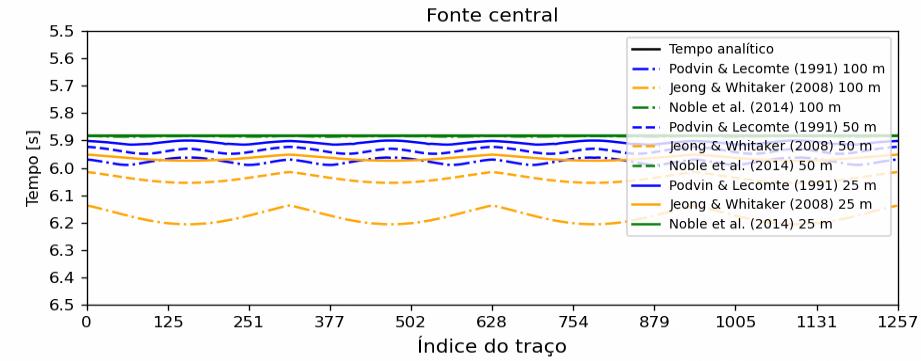
\includegraphics[width=8cm,height=3.5cm]{Imgs/RevisaoBibliografica/precision_direct.png}\label{fig:rnca}}
	\subfloat[]{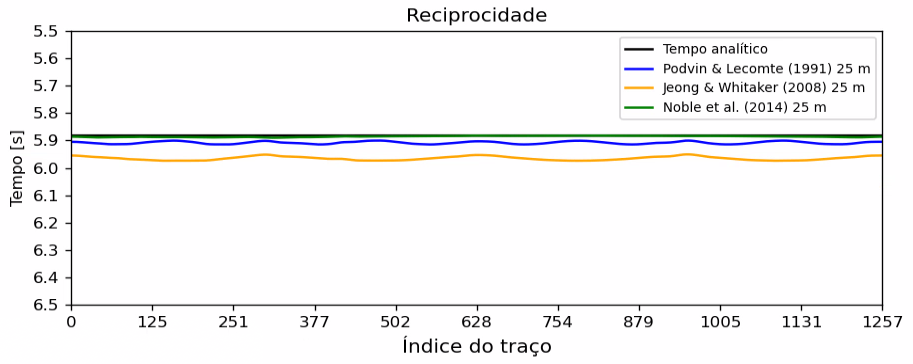
\includegraphics[width=8cm,height=3.5cm]{Imgs/RevisaoBibliografica/reciprocity.png}\label{fig:rncb}}
	
	\subfloat[]{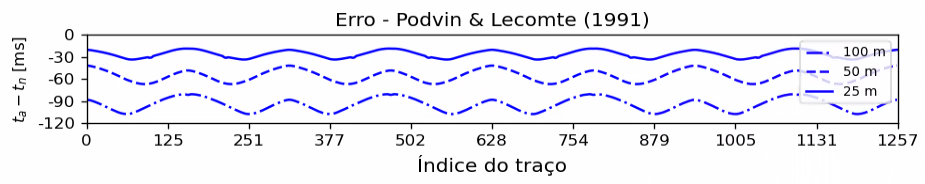
\includegraphics[width=8cm,height=1.5cm]{Imgs/RevisaoBibliografica/error_pod_direct.png}\label{fig:rncc}}
	\subfloat[]{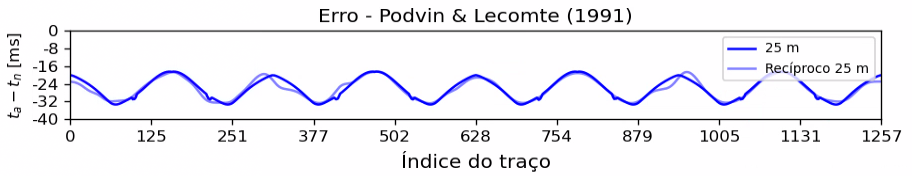
\includegraphics[width=8cm,height=1.5cm]{Imgs/RevisaoBibliografica/error_pod_reciprocity.png}\label{fig:rncd}}
	
	\subfloat[]{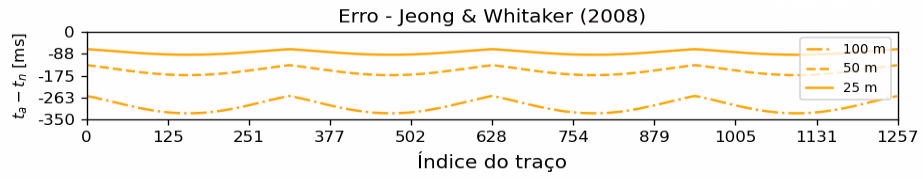
\includegraphics[width=8cm,height=1.5cm]{Imgs/RevisaoBibliografica/error_fim_direct.png}\label{fig:rnce}}
	\subfloat[]{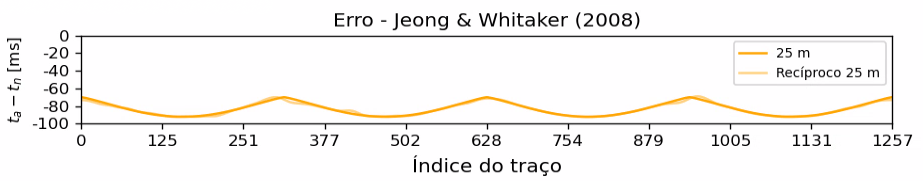
\includegraphics[width=8cm,height=1.5cm]{Imgs/RevisaoBibliografica/error_fim_reciprocity.png}\label{fig:rncf}}
	
	\subfloat[]{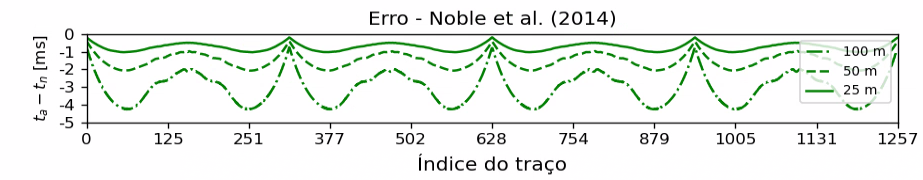
\includegraphics[width=8cm,height=1.5cm]{Imgs/RevisaoBibliografica/error_fsm_direct.png}\label{fig:rncg}}
	\subfloat[]{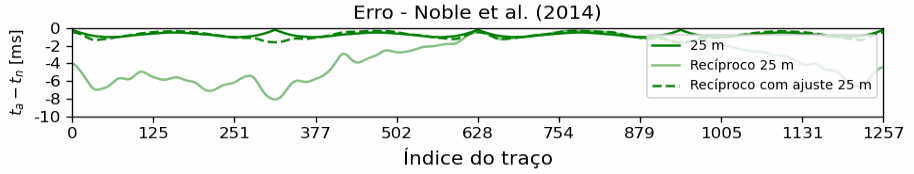
\includegraphics[width=8cm,height=1.5cm]{Imgs/RevisaoBibliografica/error_fsm_reciprocity.png}\label{fig:rnch}}
	
	\caption{Comparação de precisão entre os métodos numéricos estudados. (a) Mapeamento de todas as chegadas para os métodos numéricos testados para os espaçamentos estudados. (b) Estudo de reciprocidade utilizando o espaçamento de 25 m. (c) Escala do erro para as chegadas em diferentes espaçamentos e (d) tempo direto e recíproco utilizando a formulação de \citeonline{podvin1991finite}. (e) Escala do erro e (f) estudo de reciprocidade para a formulação de \citeonline{jeong2008fast}. (g) Escala do erro e (h) estudo de reciprocidade para a formulação de \citeonline{noble2014accurate}.}
	\label{fig:resultsNumericalComparison}
\end{figure}







\section{Inversão tomográfica}

Tipos de tomografia (reflexão, difração, transmissão e refração)







trabalhos do GISIS

\cite{santos2012tomography}
\cite{bulhoes2021efeitos}



teoria de inversão

Função objetivo e linearização

Regularização 

\cite{seo2012nonlinear}
\cite{sain2023active}



least squares conjugate gradient

\cite{saad2003iterative}




\subsection*{Tomografia de refração}

Discretização do modelo

Raios ilustrativos



\subsection*{Obtenção do dado observado}



tipos de picking (manual, analítico, machine learning)

formulação utilizada

\cite{pan2019automatic} 
\cite{qin2021first} 
